\section {DESARROLLO DE CONTENIDOS}La empresa cuenta con caracterización y tiene el propósito superior de mejorar vidas con energía sostenible y competitiva, proveer energía para que las personas de las zonas de Colombia y de los países donde operamos desarrollen su potencial y mejoren su calidad de vida. 
\\

Misión\\ 
Gestionar sistemas de transmisión, transporte y distribución, así como inversiones en el sector energético.
\\

Visión\\ 
Ser reconocidos como una empresa ética, responsable social y ambientalmente, sostenible y líder en la transición energética e innovación, logrando duplicar su EBITDA a COP 10 mil millones al 2030.
\\

Dado su proposito, esperan liderar el desarrollo, operación sostenible y rentable de la infraestructura de transmisión de energia eléctrica. Generando conexiones de progreso con nuestros grupos de interés a través de la creación de valor compartido, capitalización del conocimiento, excelencia operacional y crecimiento de las personas. 
Hay compromiso con la igualdad de oportunidades, independiente de raza, color, género, edad, estado civil, sindicación, religión, opinión política, ascendencia nacional, orientación sexual u origen social.
\\

Trabajan en 4 ejes fundamentales:\\

1.    Transmisión del Mañana

2.    Gas para el futuro

3.    Generación sostenible

4.    Ciudades Inteligentes \\

En la figura 1. podemos ver el diseño general
\begin{figure}[htb]
\centering
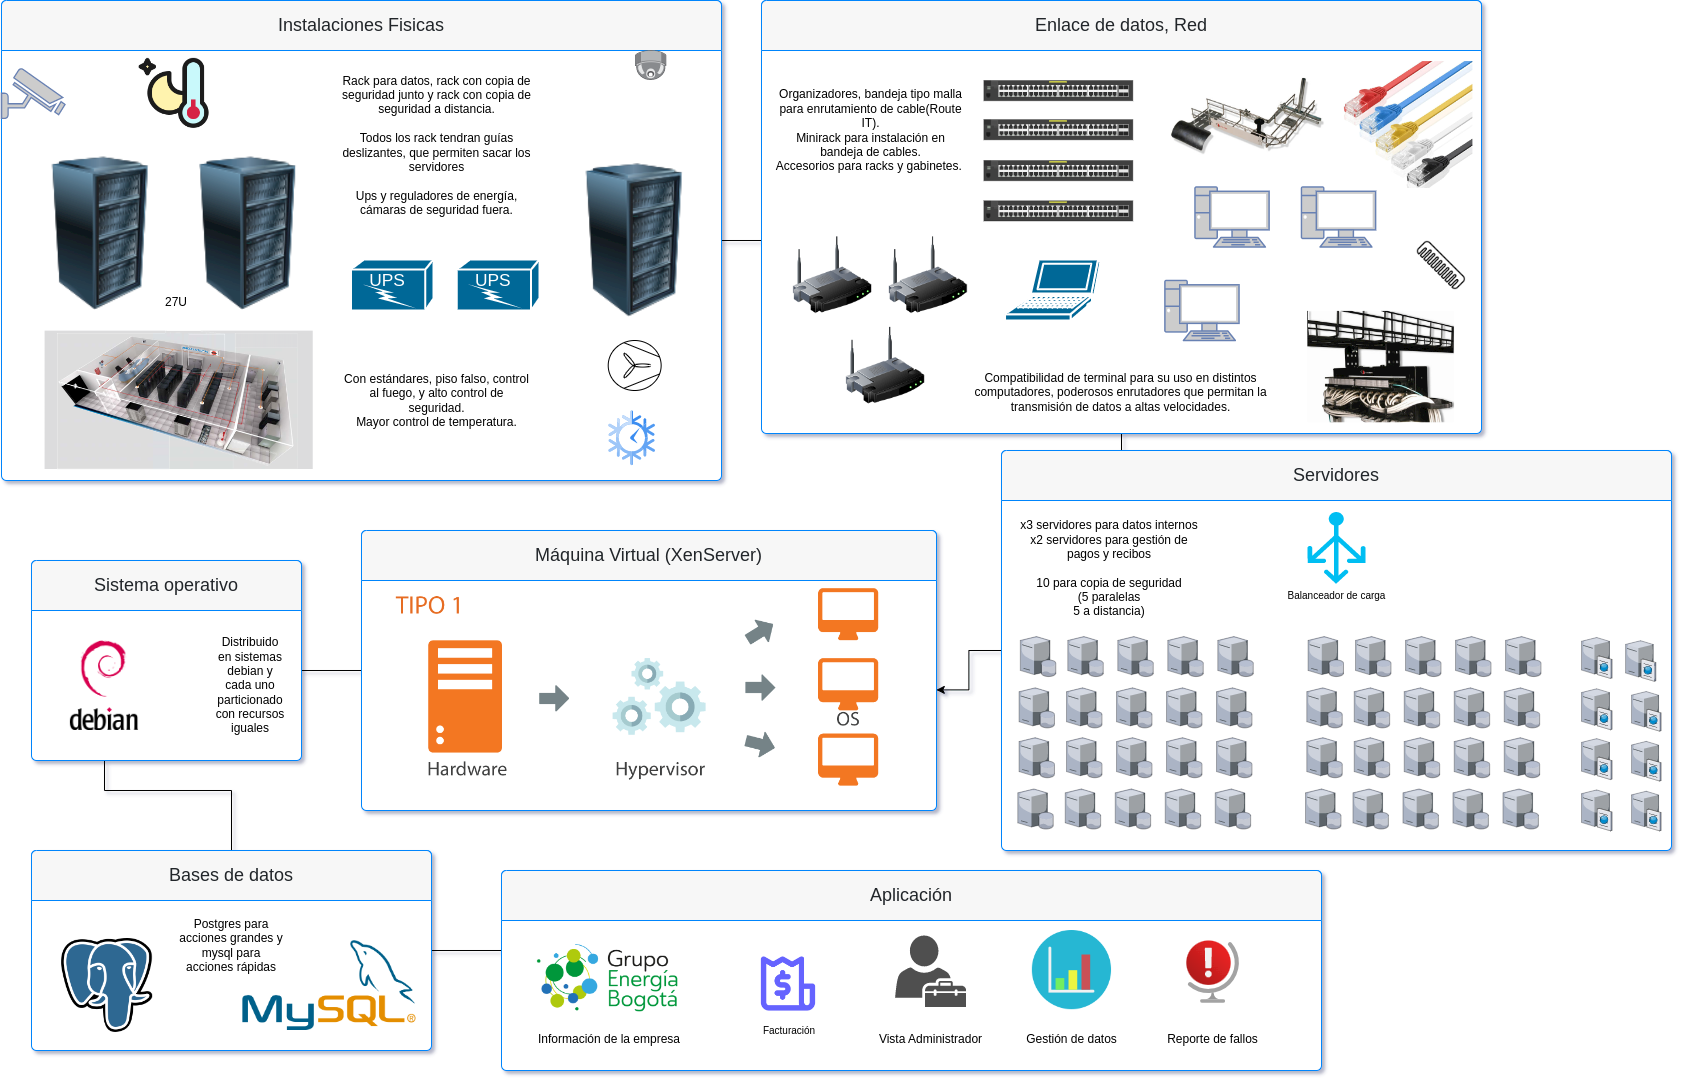
\includegraphics[width=0.5\textwidth]{assets/d.png}
\caption{Diseño general}
\label{fig:modelo}
\end{figure}
\label{sec:Background} \\

Su principal necesidad es volver a tomar el primer lugar como empresa de energía en Colombia, 
y a pesar de que tenga convenios con otros países, el problema nace al tener menos sedes en Colombia que la EPM, 
la cuál tomó el primer en el 2020. 
Las oportunidades de cumplir con la visión comenzarían al momento de extender su infraestructura por todo el país. 
Esta infraestructura tendría como principal proceso gestionar datos relacionados con el impacto 
que tendría la empresa en zonas donde no están ubicados y luego obtener mayor reconocimiento en dichos lugares 
dando uso de las TIC y fomentado su importancia. Como segundo proceso se brindará más servicios no solo de electricidad 
y gas sinó de redes que permitan acceso a información detallada en las nuevas regiones sobre las ventajas de los servicios 
enfocados a cuidar el medio ambiente, estilo vive digital. Finalmente como un tercer proceso, 
podrían extender completamente los servicios en dichas zonas con sedes colaboradoras y crear empleos 
que permitan extender aún más el nombre de la empresa en el país. Aunque este plan pueda tardar más de 5 años, 
cabe la posibilidad de que este reconocimiento acelere el proceso y puedan cumplir con la visión.  \\

En la administración de TI debe de estar en la capacidad de mantener en funcionamiento el negocio, la visión se va a medir en clientes, por lo tanto TI debe de estar en la capacidad de mantener en linea el negocio con la llegada de más clientes, brindando siempre un excelente servicio en cuanto a los servicios que ofrece la infraestructura de cómputo. \\

¿Que es multicast? \\
Acceso a la aplicación web, balanceador de carga y seguridad
El acceso a la aplicación web, lo hacen los usuarios a través de internet, donde pueden consultar detalles de facturación y hacer pago de la misma. 
Desde la administración de TI, debemos de tener en cuenta que los últimos días del mes es donde más flujo de personas habrá intentando consultar su recibo 
y por tanto estar haciendo el pago del mismo. Es importante tener claro que durante estos días el sistema no puede presentar fallos debido a que presentará inconsistencias 
en facturación ya que si los clientes no pueden realizar el pago el sistema facturará como pago tardío y aplicará mora, por lo tanto, 
esto puede generar inconvenientes con los usuarios que intentaron pagar en las fechas admitidas y quienes no pagaron en las fechas. 
Es necesario tener claro que la organización Grupo Energía Bogotá cuenta con más de 4,3 millones de clientes 
en distribución de energía eléctrica y más de 3,9 millones de clientes en distribución de gas natural, teniendo en total más de 8,2 millones de clientes.
\\ 
\\
Balanceadores de carga\\
para dar cumplimiento a las requerimientos de negocio, y teniendo en cuenta la gran cantidad de usuarios que tiene la organización y que en algunos días del mes 
se tendrá gran tráfico de peticiones a los servidores, es necesario contar con balanceadores de carga encargados de mantener altos niveles de servicio y disponibilidad 
de la plataforma web, asegurando que el tráfico web no se concentre en un solo servidor que puede generar lentitud o caída de los servicios.
Para este caso utilizaremos balanceadores de carga de tipo hardware, que consiste en servidores dedicados, cada uno con un software de balanceador de carga. 
Este servidor integra servidores web mediante soluciones plug and play, lo que significa que tan pronto se conectan, funcionan con poco o nada de ajustes previos.\\
\begin{figure}[htb]
    \centering
    \includegraphics[width=0.5\textwidth]{assets/ld1.png}
    \caption{LoadMaster XHC 100G56,727 dls}
    \label{fig:modelo}
    \end{figure}
    \label{sec:Background} \\

Precio: 56,727 dls\\
\begin{figure}[htb]
\centering
\includegraphics[width=0.5\textwidth]{assets/ca.png}
\caption{Carácteristicas}
\label{fig:modelo}
\end{figure}
\label{sec:Background} \\

Almacenamiento HDD redundante, fuente de alimentación duales, almacenamiento RAID, permite hasta 40.000 transacciones SSL por segundo 
y un rendimiento general del sistema de 90Gbit/seg, 8 puertos SFP + de 10 Gbit y 2 puertos QSFP28 de Gbit.\\

Soporte: 24 x 7 y SSO\\

Configuración: para nuestro diseño de arquitectura, optamos por tener 2 balanceadores de carga donde se deben de configurar 
para que los dos siempre estén en uso y uno adicional que entrará en funcionamiento cuando alguno vaya a entrar en mantenimiento o si llega a ocurrir un fallo.\\

Cableado :\\

cable DAC para conexiones cortas, útiles para conectar switches entre si o equipos al switch. 
Es importante tener claro que la conexión de estos cables son SFP, SFP+ o QSFP, 
por lo tanto los switches y servidores deben de ser compatibles con estos. 
Es ideal para conexiones cercanas a no más de 10 metros ya que ofrece el mismo rendimiento de los cables de fibra y sus correspondientes transceivers. 
los cables DAC son pasivos, lo que quiere decir que no contiene ningún componente activo y de alimentan directamente desde los puertos anteriormente mencionados.
balanceador de carga

    \includegraphics[width=0.5\textwidth]{assets/sp1.png}\\
    \begin{figure}[htb]
        \centering
        \includegraphics[width=0.5\textwidth]{assets/sp2.png}
        \caption{Especificaciones}
        \label{fig:modelo}
        \end{figure}
        \label{sec:Background} \\
    
        Se adjunta la imagen de el balanceador de carga
        \begin{figure}[htb]
        \centering
        \includegraphics[width=0.5\textwidth]{assets/dbc.png}
        \caption{Diseño con balanceador de carga}
        \label{fig:modelo}
        \end{figure}
        \label{sec:Background} \\

        Se adjunta la imagen del cable para transferencia de datos en Fibra Optica
        \begin{figure}[htb]
        \centering
        \includegraphics[width=0.3\textwidth]{assets/cable.png}
        \caption{Cables}
        \label{fig:modelo}
        \end{figure}
        \label{sec:Background} \\

        Cable/latiguillo/jumper de fibra óptica LC UPC a LC UPC 1m OS2 9/125 dúplex monomodo PVC (OFNR) 2.0mm
        \begin{figure}[htb]
            \centering
            \includegraphics[width=0.5\textwidth]{assets/cableA.png}
            \caption{Cables}
            \label{fig:modelo}
            \end{figure}
            \label{sec:Background} \\

            precio: 4.3 us por metro \\

            Caracteristicas: \\
            
            - chaqueta ignifuga de PVC (riser)
            - Los conectores de férula de circonio de precisión de grado A garantizan una baja pérdida
            - Las pruebas ópticas garantizan el rendimiento de la red\\


%%
%%